%%%%%%%%%%%%%%%%%%%%%%%%%%%%%%%%%%%%%
%%% THIS CHAPTER IS NOT COMPLETE! %%%
%%%%%%%%%%%%%%%%%%%%%%%%%%%%%%%%%%%%%

\chapter{Translation}
\label{ch:translation} % 4000-5000 words

% In this chapter, we describe the overall design of our solution to the problem identified in \Cref{ch:introduction}, building on work described in \Cref{ch:background}.
% TODO: Consider some kind of link from introduction

\textbf{This chapter is not complete!}

In this chapter, we discuss the translation process from C++ to Rust of the selected mini-app, HPCCG. First, we introduce the implementation details of HPCCG, along with the translation methodology undertaken. Then, we present a sequence of incrementally performant translations, showing how features of and packages for the Rust language can contribute to the performance of translations of C++ codebases. Next, we discuss approaches for the critical step of program equivalence checking to guarantee comparisons are fair. Finally, we conclude with a section on lessons learned from the process, and a proposed workflow for engineers translating High-Performance C++ codebases to Rust.

% Explain the goals of the effort
The overall goal of this effort is to generate a software product -- a Rust translation of the HPCCG codebase, with strong performance running in serial, and leveraging shared and distributed memory parallelism. On top of this, we propose a approaches for equivalence checking such translations, and use them to give confidence the Rust translation of HPCCG can be used for fair performance comparisons with the reference C++ version.

% Explain the difficulties of the effort
% No-one else has done a whole mini-app, just single kernels and toy examples
As discussed in \Cref{ch:background}, this translation effort is novel with respect to assessing High-Performance Computing for a number of reasons. Previous literature has translated only single computation kernels \cite{} with support for shared and distributed memory parallelism, or very short ``toy example'' applications of around only 150 lines \cite{} \cite{} with support for only shared memory parallelism. In contrast to this, HPCCG is a standard mini-app as part of the Mantevo suite, with the C++ version totalling 1524 lines and having support for both shared and distributed memory parallelism. This order of magnitude increase in codebase length over modern existing work \cite{}, along with support for distributed memory parallelism outside of single computation kernel contexts provides a valuable insight into the suitability of Rust in High-Performance Computing, but at the cost of significant developer effort as compared with existing work.

\section{Design}
\label{sec:translation-design} % 500 words

In traditional software development tasks, such as building the HPC MultiBench tool discussed in \Cref{ch:hpc-multibench}, system design is paramount to building a coherent product. However, for translation tasks the reference implementation has already been designed. As a result of this, the majority of the effort is in understanding the codebase to be translated, and identifying difficulties arising from the differences in program model between the original and target language.

\subsection{Differences in the Rust and C++ programming models}
\label{sec:rust-cpp-programming-models}

Every programming language can be though of as presenting a different abstraction over the capabilities of a variety of physical computer hardware. For low-level languages such as Assembly, this abstraction directly maps to the machine code instructions executed on the bare metal. Above this, languages such as C provide abstractions for common structures such as iteration, but require manual management of properties of the machine such as memory allocation. High-level scripting languages such as Python provide abstractions over memory management as well, leaving an interface very devolved from the hardware it runs on. Across many languages, the problem of program translation is reconciling these abstractions to allow the expression of the original functionality in another language.

Typically, the abstractions across programming languages are equally powerful. However, there are some caveats to this. Lambda Calculus was one of the first expressions of computation within the young field of computer science, proposed by Alonzo Church in 1933 \cite{church1932set}. Seven years later in 1940, Church proposed Simply-Typed Lambda Calculus \cite{church1940formulation}, which restricts the domain of valid programs from all programs to only well-typed ones. This is referred to as a reduction in power of the language. However, this reduction in power is beneficial to programmers, as incorrectly-typed programs are not useful. % todo: explain why/how - can't be run or internally inconsistent?

This restriction of valid programs being well-typed in Simply-Typed Lambda Calculus is mirrored by the prohibition of undefined behaviour in Rust, as shown in Figure \ref{fig:excalidraw_programs_venn}. It is beneficial to programmers, as they largely do not want to write programmers which exhibit on undefined behaviour. This is supported by the fact that programmers in other languages like C++ use dynamic and static analysis tools such as Valgrind \cite{ValgrindHome} and AddressSanitiser \cite{Sanitizers2023} to guarantee these properties outside the compiler

% TODO: Consider replacing this diagram with tikz?
\begin{figure}[H]
    \centering
    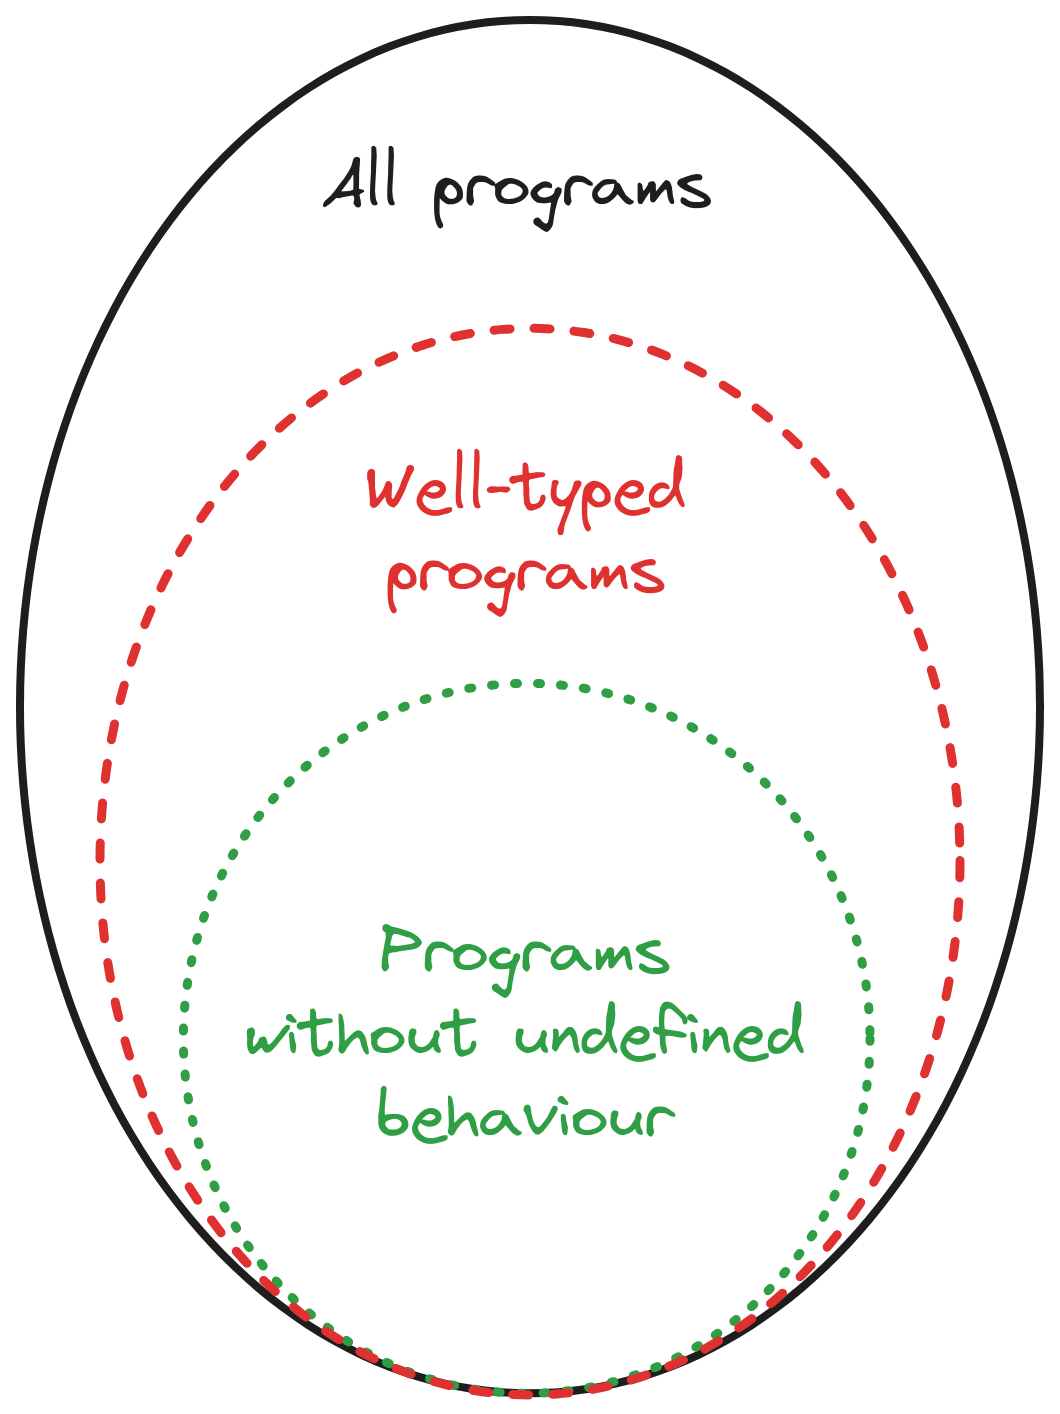
\includegraphics[width=0.5\textwidth]{images/3_translation/excalidraw_programs_venn.png}
    \caption{A diagram to show the relative powers
of increasingly restrictive program models.}
    \label{fig:excalidraw_programs_venn}
    % TODO: Check paper website for permission to reproduce
\end{figure}

When translating from languages which allow undefined behaviour such as C++ to Rust, which prohibits it my default, there are additional challenges beyond just reconciling the abstractions of the program models to express the same functionality. There are fewer safe Rust programs than C++ programs, and as a result a direct mapping to Rust may not exist if the program relies on undefined behaviour. In this case, the translation must either leverage the \mintinline{rust}{unsafe} keyword to allow such behaviour, or use a different, safe, mechanism to express the same functionality.


\subsection{Overview of HPCCG}
\label{sec:overview-hpccg}
% Overview of HPCCG

% Cite yale normally being index based
As discussed in the background to HPCCG in section \ref{ssec:hpccg}, the dominant computation kernel is an implementation of sparse matrix-vector multiplication, along with two other kernels, the vector dot product and pairwise summation of two scaled vectors. To facilitate performant implementation of these operations,
% HPCCG uses a non-standard, pointer based implementation of the traditionally index based Yale format to represent sparse matrices. % Is this actually true?
HPCCG uses a pointer based implementation of the Yale format to represent sparse matrices, which is explained through the example matrix shown in equation \ref{eq:exampleMatrix}.
% The following example describes how HPCCG uses a pointer-based variant of the compressed row storage format to represent sparse matrices.

\begin{align}
    \begin{pmatrix}
        0 & 1 & 0 & 2 \\
        0 & 0 & 5 & 0 \\
        0 & 4 & 6 & 0 \\
        3 & 0 & 0 & 0
    \end{pmatrix}
    \label{eq:exampleMatrix}
\end{align}

A sparse matrix can then be represented as two nested lists -- one containing the non-zero values in each row, and the other the indices of those non-zero values in that row. This means the sparse matrix in (\ref{eq:exampleMatrix}) can be written as:

\begin{verbatim}
list_of_vals = [   [1, 2]  ,  [5]  ,  [4, 6]  ,  [3]   ]
list_of_inds = [   [1, 3]  ,  [2]  ,  [1, 2]  ,  [0]   ]
\end{verbatim}
% \begin{align}
%     \verb!list_of_vals = [   [1, 2]  ,  [5]  ,  [4, 6]  ,  [3]   ]! \\
%     \verb!list_of_inds = [   [1, 3]  ,  [2]  ,  [1, 2]  ,  [0]   ]!
%     \label{eq:exampleMatrixRepr}
% \end{align}

This structure uses much less memory, but has the drawback that the inner lists for each row are of variable length, making the outer list non-homogenous. HPCCG's data structure is a flattening of the above structure to use single-dimensional arrays rather than nested ones for \texttt{list\_of\_vals} and \texttt{list\_of\_inds}. This then requires a mechanism to distinguish rows, so it uses auxiliary data structures for the lengths of each row (an array of integers called \texttt{nnz\_in\_row}), along with pointers to the start of each row in the values and indices arrays (two arrays of pointers called \texttt{ptr\_to\_vals\_in\_row} and \texttt{ptr\_to\_inds\_in\_row} respectively). Finally, the number of rows (an integer called \texttt{total\_nrow}) is also needed. Hence, HPCCG would represent the sparse matrix in (\ref{eq:exampleMatrix}) as follows:

\begin{verbatim}
total_nrow          = 4
nnz_in_row          = [ 2 ,     1 , 2 ,     1 ]
list_of_vals        = [ 1 , 2 , 5 , 4 , 6 , 3 ]
ptr_to_vals_in_row  = [ ↑ ,     ↑ , ↑,      ↑ ]
list_of_inds        = [ 1 , 3 , 2 , 1 , 2 , 0 ]
ptr_to_inds_in_row  = [ ↑ ,     ↑ , ↑,      ↑ ]
\end{verbatim}

To traverse the values in a row $i$ of this data structure, first retrieve the pointer to the starting point in the list of values from \texttt{ptr\_to\_vals\_in\_row[i]}. Then, traverse through the list of values for the number of non-zeroes, \texttt{nnz\_in\_row[i]}. This same process applies to traversing indices in a row.

This data structure provides significant performance improvements over a full matrix representation for the sparse matrix-vector multiplication operation. This is because it minimises both the memory bandwidth and arithmetic operations required, by omitting the zero-values which would not contribute to the product.

Unfortunately, this pointer based implementation presents difficulties when translating to Rust, as operations on raw pointers considered unsafe, as the borrower checker is less able to reason about their memory safety. This difficulty is addressed in the first two translation versions, \ref{sec:translation-direct} and \ref{sec:translation-direct}.


\section{Implementation}
\label{sec:translation-implementation} % 3000 words

This section provides a description of the technical details of the translation process. In order to guarantee that the Rust implementation is performant as possible, and hence representative of the capabilities of the Rust language, a workflow of incremental improvement wsa adopted for the translation process. First, a direct translation to Rust was undertaken, matching the program model as closely as possible to provide confidence in program equivalence. Then, a number of incremental improvements to the Rust implementation were undertaken to result in a performant serial implementation of the HPCCG mini-app. Then, this serial implementation was modified to implement shared and distributed memory parallelism using Rayon and the Rust MPI bindings. Source code for each of these translation versions can be found in the \texttt{hpccg-rs} GitHub repository.


\subsection{Direct translation}
\label{sec:translation-direct}
% Naive translation + explaining Rust ownership and borrowing

The first translation was designed to be as direct a mapping between the program models of C++ and Rust as possible. This helped develop a strong understanding of the codebase, and gave initial confidence in program equivalence, as the only factor which could affect program functionality is the language semantics of Rust differing from C++.

In C and C++, pointers for memory indirection are incredibly ubiquitous. This is especially true in High-Performance computing, where codebases often operate on multi-dimensional arrays representing meshes, which are represented in C++ by pointers. However, using pointers in this way makes programs very susceptible to bugs, for example accessing uninitialised memory as a result of faulty pointer arithmetic. As discussed in section \ref{ssec:rust-indirection}, which covered memory indirection in Rust, interaction with raw pointers in Rust is considered an \mintinline{rust}{unsafe} operation, as it is difficult to statically guarantee that it will not result in undefined behaviour. Much of the behaviour of pointers can instead be implemented through borrowing. However, the borrow checker is overly restrictive for some use cases, requiring the use of smart pointers.

This presented the first significant challenge in the translation effort, as the implementation of the Yale representation of sparse matrix in HPCCG relies heavily on raw pointers and pointer arithmetic. This complicates the direct translation process, as references and smart pointers in Rust necessarily have different semantics to raw pointers, and may be less performant. This was identified as a risk during the specification phase, and was captured in the Risk Matrix \ref{tab:risk_matrix}, which is shown in \Cref{ch:project-management} in the discussion of project management. A truncated version of the data structure which implements this Yale representation in C++ is shown in Listing \ref{listing:cpp-sparse-matrix-structure}.

\begin{listing}[H]
    \begin{minted}[linenos,breaklines]{c++}
struct HPC_Sparse_Matrix_STRUCT {
  int total_nrow;
  long long total_nnz;
  int  * nnz_in_row;
  double ** ptr_to_vals_in_row;
  int ** ptr_to_inds_in_row;
  double ** ptr_to_diags;
  double *list_of_vals;
  int *list_of_inds;
}
    \end{minted}
    \caption{A truncated version of the C++ data structure which implements the Yale representation of the sparse matrix, from Heroux's original implementation of HPCCG \cite{MantevoHPCCG2023}.}
    \label{listing:cpp-sparse-matrix-structure}
\end{listing}

This data structure must then be populated to the initial configuration of the conjugate gradient problem, with the reference C++ implementation shown in Listing \ref{listing:cpp-sparse-matrix-structure-population}. This process presents a challenge to the translation process, not only because it dereferences raw pointers, but also it violates Rust's ownership rules, as there are concurrent mutable and immutable pointers to the data, for example lines 7 and 17 in Listing \ref{listing:cpp-sparse-matrix-structure-population}.

\begin{listing}[H]
    \begin{minted}[linenos,breaklines]{c++}
for (int iz=0; iz<nz; iz++) {
    for (int iy=0; iy<ny; iy++) {
        for (int ix=0; ix<nx; ix++) {
        int curlocalrow = iz*nx*ny+iy*nx+ix;
        int currow = start_row+iz*nx*ny+iy*nx+ix;
        int nnzrow = 0;
        (*A)->ptr_to_vals_in_row[curlocalrow] = curvalptr;
        (*A)->ptr_to_inds_in_row[curlocalrow] = curindptr;
        for (int sz=-1; sz<=1; sz++) {
            for (int sy=-1; sy<=1; sy++) {
                for (int sx=-1; sx<=1; sx++) {
                    int curcol = currow+sz*nx*ny+sy*nx+sx;
                        if ((ix+sx>=0) && (ix+sx<nx) && (iy+sy>=0) && (iy+sy<ny) && (curcol>=0 && curcol<total_nrow)) {
                            if (!use_7pt_stencil || (sz*sz+sy*sy+sx*sx<=1)) {
                                if (curcol==currow) {
                                    *curvalptr++ = 27.0;
                                } else {
                                    *curvalptr++ = -1.0;
                                }
                                *curindptr++ = curcol;
                                nnzrow++;
                            } 
                        }
                }
            }
        }
        (*A)->nnz_in_row[curlocalrow] = nnzrow;
        nnzglobal += nnzrow;
        (*x)[curlocalrow] = 0.0;
        (*b)[curlocalrow] = 27.0 - ((double) (nnzrow-1));
        (*xexact)[curlocalrow] = 1.0;
        }
    }
}
    \end{minted}
    \caption{A truncated version of the C++ function to populate the initial configuration of the sparse matrix, from Heroux's original implementation of HPCCG \cite{MantevoHPCCG2023}.}
    \label{listing:cpp-sparse-matrix-structure-population}
\end{listing}

This code snippet exemplifies how HPCCG is not a single computational kernel, nor a toy example, but a mini-app representative of structural complexities in full-scale applications for High-Performance Computing.

The first key insight in the translation process is that the interior mutability pattern of smart pointers, discussed in section 15-5 of the Rust book \cite{RustProgrammingLanguage} can be used to represent this functionality, despite the presence of concurrent mutable and immutable pointers to the data. Instead of arrays of pointers such as \mintinline{c++}{int ** ptr_to_inds_in_row} as shown in Listing \ref{listing:cpp-sparse-matrix-structure}, the \mintinline{rust}{Rc<RefCell<f64>>} construct can be used to create a vector of items which allow concurrent mutable and immutable borrows. This works by presenting a safe interface to an \mintinline{rust}{unsafe} implementations which performs checks at runtime to guarantee memory safety. As such, the data structure shown in Listing \ref{listing:cpp-sparse-matrix-structure} can be re-written in Rust, as shown in Listing \ref{listing:rust-sparse-matrix-structure}.

\begin{listing}[H]
    \begin{minted}[linenos,breaklines]{rust}
#[derive(Debug)]
pub struct SparseMatrix {
    pub total_nrow: i32,
    pub total_nnz: i32,
    pub nnz_in_row: Vec<i64>,
    pub ptr_to_vals_in_row: Vec<Rc<RefCell<f64>>>,
    pub ptr_to_inds_in_row: Vec<Rc<RefCell<i32>>>,
    pub list_of_vals: Vec<Rc<RefCell<f64>>>,
    pub list_of_inds: Vec<Rc<RefCell<i32>>>,
}
    \end{minted}
    \caption{A truncated version of the sparse matrix data structure, directly translated to Rust using the interior mutability pattern of smart pointers.}
    \label{listing:rust-sparse-matrix-structure}
\end{listing}

As discussed in \Cref{ch:background}, the dominant computational kernel of HPCCG is sparse matrix-vector computation. Listing \ref{} shows how this is implemented leveraging the Yale sparse matrix representation outlined in Listing \ref{listing:cpp-sparse-matrix-structure}.

\begin{listing}[H]
    \begin{minted}[linenos,breaklines]{c++}
int HPC_sparsemv( HPC_Sparse_Matrix *A, const double * const x, double * const y) {
  const int nrow = (const int) A->local_nrow;
  for (int i=0; i< nrow; i++) {
      double sum = 0.0;
      const double * const cur_vals = 
     (const double * const) A->ptr_to_vals_in_row[i];
      const int    * const cur_inds = 
     (const int    * const) A->ptr_to_inds_in_row[i];
      const int cur_nnz = (const int) A->nnz_in_row[i];
      for (int j=0; j< cur_nnz; j++) {
        sum += cur_vals[j]*x[cur_inds[j]];
      }
      y[i] = sum;
    }
  return(0);
}
    \end{minted}
    \caption{The C++ function to compute sparse matrix-vector multiplication, from Heroux's original implementatino of HPCCG \cite{MantevoHPCCG2023}.}
    \label{listing:cpp-sparsemv}
\end{listing}

Having implemented the data structure leveraging the interior mutability pattern as shown in Listing \ref{listing:rust-sparse-matrix-structure}, this sparse matrix-vector kernel can be translated to Rust, as shown in Listing \ref{listing:rust-sparsemv-direct}. Here, we can see the structural similarities between the original code and the translation, but also instances where smart pointers introduce extra boilerplate, such as the \mintinline{rust}{borrow} function on lines 9 and 10.

\begin{listing}[H]
    \begin{minted}[linenos,breaklines]{rust}
pub fn sparsemv(matrix: &SparseMatrix, vector: &[f64]) -> Vec<f64> {
    let nrow = matrix.local_nrow as usize;
    let mut y = Vec::with_capacity(vector.len());
    let mut start_index = 0;
    for i in 0..nrow {
        let mut sum = 0.0;
        let cur_nnz = matrix.nnz_in_row[i] as usize;
        for j in 0..cur_nnz {
            let val = *matrix.list_of_vals[start_index + j].borrow();
            let ind = *matrix.list_of_inds[start_index + j].borrow() as usize;
            sum += val * vector[ind];
        }
        y.push(sum);
        start_index += cur_nnz;
    }
    y
}
    \end{minted}
    \caption{A direct translation to Rust of the C++ function to compute sparse matrix-vector multiplication.}
    \label{listing:rust-sparsemv-direct}
\end{listing}

There are two other computational kernels in HPCCG: calculating a vector dot product, and pairwise summation of two scaled vectors. However, as discussed in \Cref{ch:background}, these take up a much smaller proportion of the runtime than the sparse matrix-vector multiplication. In addition to this, they present significantly less challenge with respect to translation, as they are dependent only on C++ arrays which can be implemented in Rust through the \mintinline{rust}{Vec} type, rather than a custom data structure of pointers as with the sparse matrix representation.

Unfortunately, leveraging the interior mutability pattern comes at a steep cost to performance, as the guarantees against undefined behaviour are deferred to runtime, meaning every pointer dereference must be bounds checked, doubling the instruction count per dereference. This can be seen in Figure \ref{fig:perf_annot_labelled}, which shows a screenshot of the \texttt{perf} performance profiler, which is introduced in more depth in \ref{ssec:perf profiler}.

\begin{figure}[H]
    \centering
    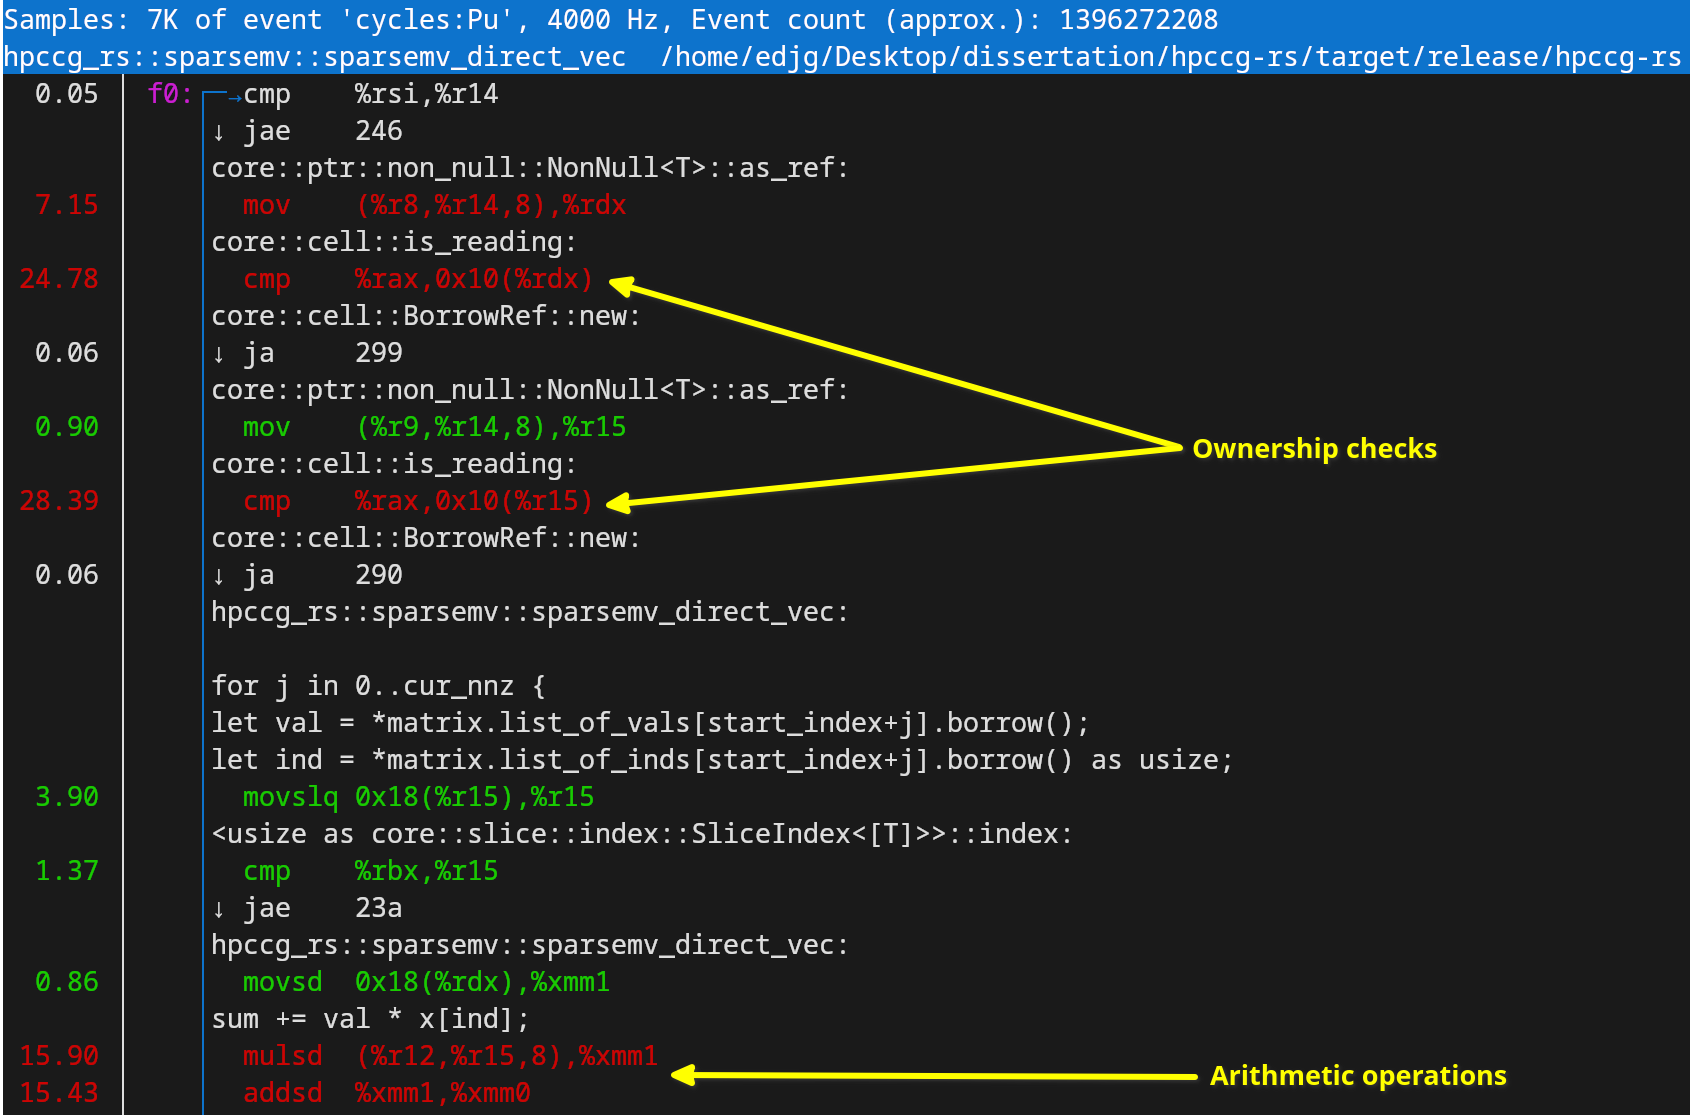
\includegraphics[width=0.75\textwidth]{images/3_translation/perf_annot_labelled.png}
    \caption{An annotated screenshot of the \texttt{perf} performance profiler, showing the dominating performance impact of extra instructions checking the dereference operation.}
    \label{fig:perf_annot_labelled}
\end{figure}

This performance cost is unacceptable for High-Performance Computing use cases. Hence, for Rust to be viable for these purposes, there must be a way to avoid incurring this cost.

\subsection{Reworked data structure}
\label{sec:translation-reworked-data-structure}
% Restructured data structure

Having made a direct translation of HPCCG into Rust, the next step was to incrementally improve it by modifying the implementation to use a data structure more amenable to Rust's program model.

In Rust, there are many constraints placed on the use of pointers, due to the difficulty to reason about them and their memory safety at compile time. In HPCCG, pointers are exclusively used to define arrays, and to point into positions in other arrays. In addition to this, there are fewer semantic restrictions on indexes in Rust than raw pointers or borrowed references, as they are restricted to the specific domain of accessing arrays, rather than the many use cases pointers support. As a result of this, it was decided to re-work the Yale representation data structure of the sparse matrix to use indexing as opposed to pointers.

As part of its rich type system, the Rust language provides a data type specific to data used as indexes, called \mintinline{rust}{usize}. The amount of data stored by this type depends on the address space of the machine it is compiled on, with 32-bit architectures having the same domain as the \mintinline{rust}{u32} -- an unsigned 32 bit integer, and 64-bit architectures having the same domain as \mintinline{rust}{u64}. This guarantees that any length of array can be indexed by this type, but also differentiates data which is used as an index from other data, allowing developers to more intuitively understand the meaning of code through its type system.

This switch to using and index, rather than pointer, based implementation is shown in Listing \ref{listing:rust-sparse-matrix-structure-indexed}, which contrasts the direct Rust translation shown in Listing \ref{listing:rust-sparse-matrix-structure}. This change also reduces the complexity of the implementation to populate the initial configuration of the sparse matrix. In the index based structure, only the vector \mintinline{rust}{push} and indexing operations are required, whereas the direct translation using smart pointers also requires careful use of the \mintinline{rust}{borrow_mut} and \mintinline{rust}{clone} operations. This reduces the total wall time required to run the program, which includes the time to populate the initial configurations for the mini-app.

In addition to this, a second key insight is that the pointers in the \texttt{ptr\_to\_vals\_in\_row} and \texttt{ptr\_to\_inds\_in\_row} both reference the same indices, just in different arrays at different memory addresses. As a result of this, only a single vector of indices is required, rather than two arrays of pointers. This slightly reduces the memory bandwidth required to transfer the sparse matrix, which may increase performance in memory-bound workloads, as discussed in section \ref{sssec:roofline-models} of \Cref{ch:performance}.

\begin{listing}[H]
    \begin{minted}[linenos,breaklines]{rust}
#[derive(Debug)]
pub struct SparseMatrix {
    pub total_nrow: usize,
    pub total_nnz: usize,
    pub nnz_in_row: Vec<usize>,
    pub row_start_inds: Vec<usize>,
    pub list_of_vals: Vec<f64>,
    pub list_of_inds: Vec<usize>,
}
    \end{minted}
    \caption{A truncated version of the sparse matrix data structure, re-worked in Rust to use an index rather than pointer based implementation of the Yale representation.}
    \label{listing:rust-sparse-matrix-structure-indexed}
\end{listing}

% TODO: Section about sparsemv
Having adopted this index based approach to the sparse matrix data structure, the implementation of the sparse matrix-vector operation must also be modified. The updated implementation, shown in Listing \ref{listing:rust-sparsemv-indexed}, is structurally very similar to the implementation in the direct translation, shown in Listing \ref{listing:rust-sparsemv-direct}. The main differences are in how values in the sparse matrix are accessed, through a single index accessed on line 6, then re-used across lines 9 and 10, rather than two individual pointers which are then both dereferenced.

\begin{listing}[H]
    \begin{minted}[linenos,breaklines]{rust}
pub fn sparsemv(matrix: &SparseMatrix, vector: &[f64]) -> Vec<f64> {
    let nrow = matrix.local_nrow;
    let mut result = Vec::with_capacity(vector.len());
    for i in 0..nrow {
        let mut sum = 0.0;
        let start_ind = matrix.row_start_inds[i];
        let cur_nnz = matrix.nnz_in_row[i];
        for j in 0..cur_nnz {
            sum += matrix.list_of_vals[start_ind + j]
                * vector[matrix.list_of_inds[start_ind + j]];
        }
        result.push(sum);
    }
    result
}
    \end{minted}
    \caption{A translation to Rust of the C++ function, using a single-indexed sparse matrix representation to compute sparse matrix-vector multiplication.}
    \label{listing:rust-sparsemv-indexed}
\end{listing}

The implementations of the other two computational kernels, calculating a vector dot product and pairwise summation of two scaled vectors, remain unchanged -- as neither of them interact with the sparse matrix implementation.

% Insert figure comparing indexed with direct translation through HPC MultiBench
% Total wall time, and just the sparsemv and ddot kernels?

Since High-Performance Computing workloads are often array or mesh based, this strategy of replacing pointers with indices still holds for the dominant computational kernels of many full applications. Where pointers cannot be substituted with indices, borrowed references should be preferred, then smart pointers such as the \mintinline{rust}{Rc<RefCell<f64>>} construct as a worst-case solution.

\subsection{Bounds checking}
\label{sec:translation-bounds-checking}
% Bounds checking
% Discussion of bounds checking in rust

In Rust, all array indexing operations are bounds checked by default, to guarantee memory safety. This incurs a performance cost as a result of this comparison operation, and any resultant pipeline stalls as a result of it. As a result of this, the default indexing strategy in Rust is around twice as slow as in languages without these checks, such as C++. This result is explained in depth in section \ref{ssec:perf-profiler} of \Cref{ch:performance}, as part of a discussion of the \texttt{perf} performance profiler.

% How to get around it
Fortunately, Rust provides a mechanism to disable these runtime checks -- the \texttt{get\_unchecked} function on vectors. However, this function is necessarily \mintinline{rust}{unsafe}, as it could result in accessing uninitialised memory if the programmer provides an index beyond the size of the vector. Listing \ref{listing:rust-sparsemv-unchecked} shows an implementation again using the indexed sparse matrix representation, but this time with unchecked indexing.

\begin{listing}[H]
    \begin{minted}[linenos,breaklines]{rust}
pub fn sparsemv(matrix: &SparseMatrix, vector: &[f64]) -> Vec<f64> {
    let nrow = matrix.local_nrow;
    let mut result = Vec::with_capacity(vector.len());
    for i in 0..nrow {
        let mut sum = 0.0;
        let start_ind = unsafe { *matrix.row_start_inds.get_unchecked(i) };
        let cur_nnz = unsafe { *matrix.nnz_in_row.get_unchecked(i) };
        for j in 0..cur_nnz {
            sum += unsafe {
                matrix.list_of_vals.get_unchecked(start_ind + j)
                    * vector.get_unchecked(*matrix.list_of_inds.get_unchecked(start_ind + j))
            };
        }
        result.push(sum);
    }
    result
}
    \end{minted}
    \caption{A translation to Rust of the C++ function, using unchecked vector indexing to compute sparse matrix-vector multiplication.}
    \label{listing:rust-sparsemv-unchecked}
\end{listing}

% Figures comparing performance

However, this approach nullifies Rust's beneficial property of guaranteeing memory safety. We are disabling runtime checks of indexes to gain performance, and hence regressing back to C++ with the only guarantees of memory safety being through programmer confidence. However, the Rust language provides syntax sugars in the form or zero-cost abstractions which can help avoid these unsafe operations in common use cases.

\subsection{Iterators}
\label{sec:translation-iterators}
% Iterators

A key feature of Rust is zero-cost abstractions

% Using iterators for HPCCG

% Figures comparing performance

Although in this case the use of iterators does not eliminate the need for unchecked array indexing, it reduces the number of instances of their use, which reduces the surface for possible invalid memory access within a program. It is possible to construct nested iterators such that only one unchecked index operation is required -- which cannot be removed as it is part of the data in the sparse matrix representation, and doesn't range over a known set of values. However, this was not done in this implementation to make the implementation more amenable to the use of Rayon for shared memory parallelism.

\subsection{Shared memory parallelism}
\label{sec:translation-rayon}
% Shared-memory parallelism with Rayon

Having modified the Rust implementation to leverage iterators, it is incredibly easy to leverage shared memory parallelism through Rayon. The only change required is replacing instances of the native Rust \texttt{iter} function with the \texttt{par\_iter} function provided by Rayon.

% TODO: Consider moving this to be in the background section `Fearless Parallelism`
% Introducing rayon over thread primitives

% Using iterators for HPCCG
Listing \ref{} shows the implementation of the sparse matrix-vector multiplication kernel. This change to leveraging shared memory parallelism requires only two eight characters to be changed -- adding the \texttt{par} prefix to the two outer zipped iterators. In addition to this, as a result of the Rust compiler's static checks, there are much stronger guarantees against data races. Section \ref{ssec:shared-memory-paralellism} of \Cref{ch:background} showed how easy it is to introduce a data race using OpenMP even for a trivial example. However, the ownership constraints and scoping rules of closures for functions over iterators ensure that data cannot be concurrently accessed across threads.

The combination of these two factors, ease of switching to multi-threading and guarantees of correctness, empowers developers to quickly write performant code by leveraging shared memory parallelism.

% Figures comparing performance

In summary, the use of packages such as Rayon allows developers to write multi-threaded Rust code incredibly quickly, and with confidence in its correctness. Due to the current trend in hardware design towards multi-processor architectures in machines discussed in \Cref{ch:background}, this allows developers to fully leverage the performance of commodity hardware, which is crucial in a High-Performance Computing context.

\subsection{Distributed memory parallelism}
\label{sec:translation-mpi}
% Distributed-memory parallelism with rs-mpi

% Introducing MPI

The process of translating the MPI aspect of HPCCG into Rust was by far the most difficult part of the translation process. It was significantly more complex than the next most difficult aspect of populating the data structure -- taking around two weeks instead of two days of dedicated work. This difficulty was broadly as a result of three key factors:

\begin{enumerate}
    \item The length of the codebase to translate -- the \texttt{make\_local\_matrix.cpp} file alone is 612 lines long
    \item The imperfect mapping between the C++ MPI calls and the Rust MPI bindings
    \item The poor documentation of the Rust MPI bindings
\end{enumerate}

% Rust bindings into MPI (+ poor documentation, link to future open source work)

% Translation effort snippets

% Performance

% Summarise final result of all translation
In summary, the translation effort resulted in a performant implementation of the HPCCG mini-app in Rust, supporting both shared-memory parallelism through Rayon, along with the stretch goal of distributed memory parallelism through the Rust MPI bindings. This demonstrates that it is possible to use Rust for High-Performance Applications, which HPCCG is representative of. However, there are still aspects of Rust which add difficulty to this process, such as the state of the documentation of the Rust bindings to MPI -- but this is likely to improve in the future as Rust and its ecosystem matures.





\section{Equivalence checking}
\label{sec:equivalence-checking} % 3000 words

Equivalence checking is critical to make performance comparisons between programs fair. In order to draw conclusions about the performance of the Rust translation of HPCCG, there must be strong confidence that it provides the same functionality as the C++ version. Taking this to its logical extremes, a Rust program which immediately terminates will have a much lower total runtime than the C++ implementation of HPPCG, but it clearly would not be a fair comparison of Rust and C++. However, the usefulness of equivalence checking is not only for ensuring performance comparisons are fair. Any translation effort from existing C++ code to Rust 

As a result of this, a significant part of this project is developing techniques and workflows to equivalence check

\subsection{End-to-end testing}
\label{sec:equivalence-end-to-end}
% end-to-end testing

The simplest form of equivalence checking is end-to-end testing. This refers to running programs with the same input data, and asserting that they yield the same outputs.

\subsection{Formal methods}
\label{sec:equivalence-end-to-end}
% formal methods (and why they aren't suitable)

\subsection{Assembly and IR analysis}
\label{sec:equivalence-end-to-end}
% LLVM analysis (and why it is hard to scale)

\subsection{Unit testing}
\label{sec:equivalence-unit-testing}
% Unit testing

\subsubsection{Test driven development}
\label{sec:equivalence-tdd}

Test-driven development refers to


\subsection{A novel approach}
\label{sec:equivalence-polyglotest}
% polyglotest approach



% % TODO: Could omit this, it's an interesting aside, but if stuff needs to be cut, this is it
% \section{Supply-side verification}
% \label{sec:translation-supply-side-verification} % 500 words
% % Why is this important?
% % `cargo vet`


% % TODO: Could omit this, it's an interesting aside, but if stuff needs to be cut, this is it
% \subsection{Non-determinism in HPCCG}
% \label{sec:hpccg-race-conditions}
% % Explain uncommon bug resulting in non-deterministic results in HPCCG


\section{Lessons learned and proposed workflow}
\label{sec:translation-workflow}